В роли управляющего компонента стенда выступает система на кристалле Xilinx ZYNQ-7000 XC7Z020 CLG400, являющаяся объединением процессорной системы и программируемой логики. Архитектура данного кристалла представлена на рисунке \ref{fig:Arch_XC7Z020}.\par
\begin{figure}[ht]
    \centering
    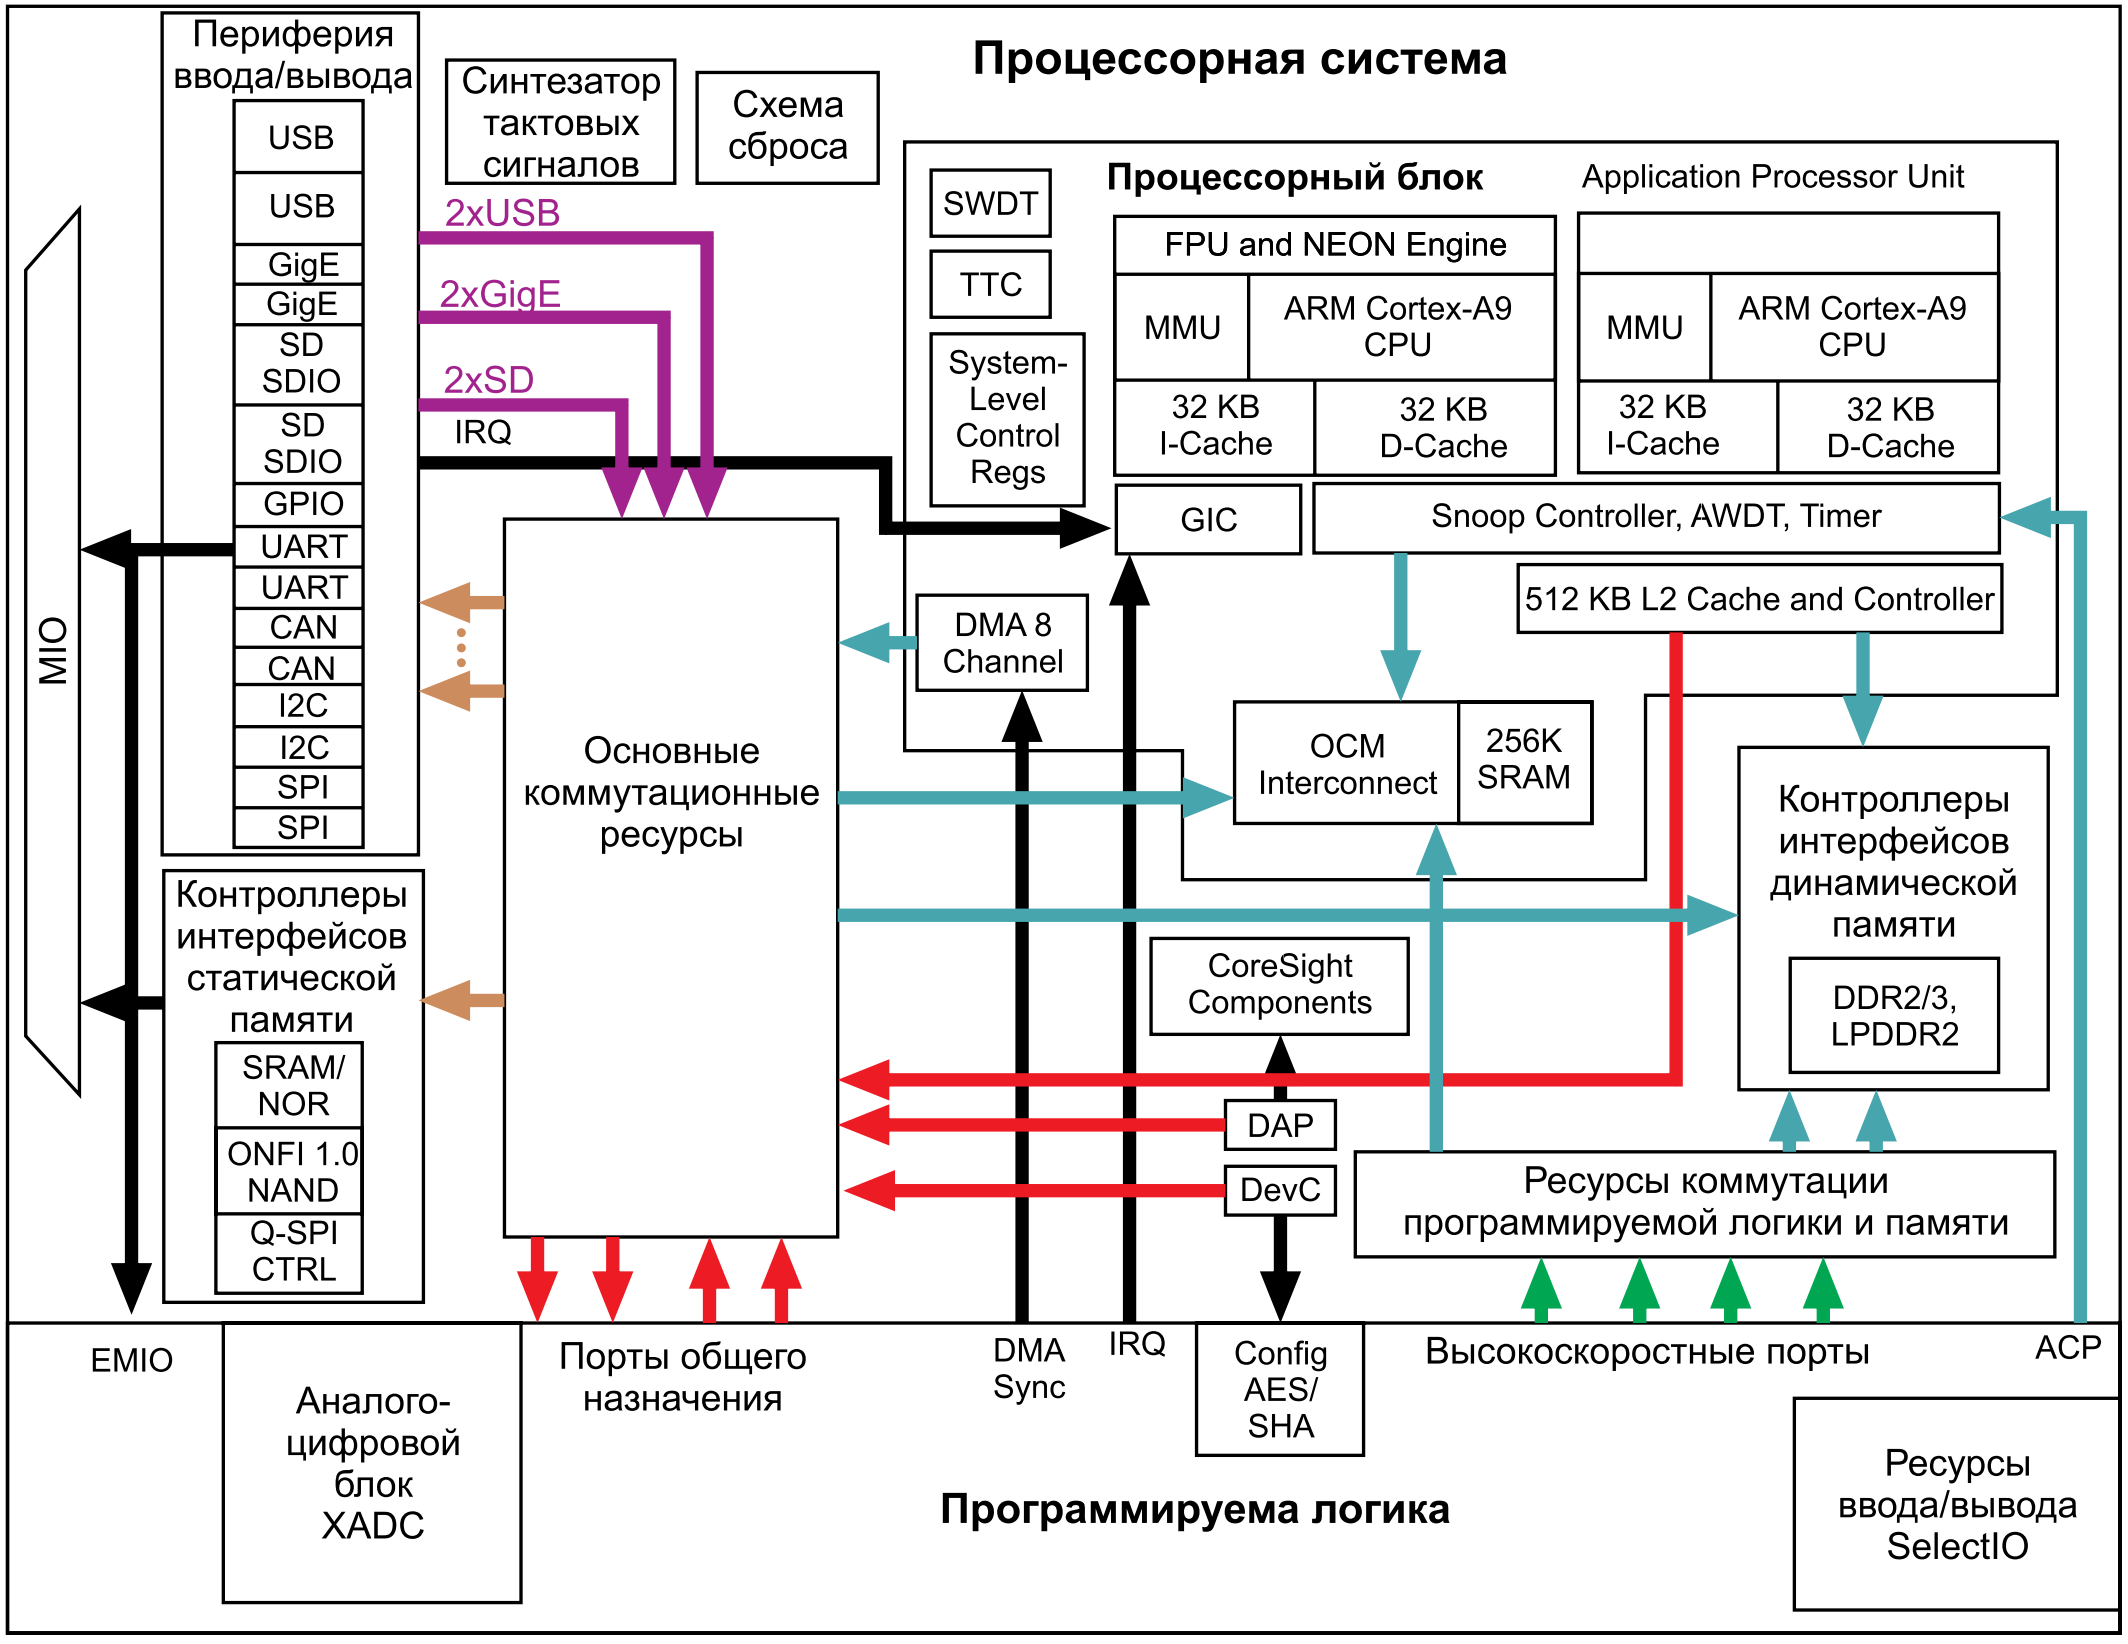
\includegraphics[width=1\linewidth]{Arch_XC7Z020.png}
    \caption{Архитектура программируемой системы на кристалле XC7Z020}
    \label{fig:Arch_XC7Z020}
\end{figure}
Процессорная система реализована на базе аппаратного блока, включающего в себя два ядра ARM Cortex-A9 MPCore \parencite{Cortex-A9}, кэш-память первого и второго уровней объёмом 32 и 512 кбайт соответственно. В качестве оперативной памяти присутствует внутрикристалльное ОЗУ ёмкостью 256 кбайт, а также контроллер внешней высокоскоростной оперативной динамической памяти, поддерживающий многие современные спецификации. Периферия ввода/вывода включает в себя интерфейсы USB 2.0, Tri-mode Gigabit Ethernet, SD/SDIO, UART, CAN 2.0, I2C и SPI, каждый из которых реализован дважды.\par
Программируемая логика данной системы на кристалле близка к ПЛИС семейства Artix-7. Это решение включает в себя 87040 логических ячеек, 140 модулей памяти Block RAM общей ёмкостью 560 кбайт, 220 секций цифровой обработки сигналов DSP48E1 и один аналогово-цифровой блок XADC.\par
Взаимодействие двух рассмотренных частей: программируемой логики и процессорной системы осуществляется через порты шины AXI \parencite{AXI}. Данная шина имеет 3 интерфейса:
\begin{itemize}
    \item AXI4 --- для высокопроизводительной работы с устройствами, отображаемых на адресное пространство памяти;
    \item AXI4-Lite --- для простой, низкоскоростной связи с переферийными устройствами, не имеющих высоких требований к пропускной способности(например, для регистров управления и состояния);
    \item AXI4-Stream --- для высокоскоростной потоковой передачи данных.
\end{itemize}\par
Система на кристалле даёт возможность одновременно использовать преимущества процессорных вычислений и параллельной обработки данных программируемой логики.
